\chapter{Konzept}
\label{chap:konzept}


\section{Allgmein}
Bei der Beschreibung eines Devices werden folgende drei Bereiche unterschieden:


\textbf{State:} \\
Die Menge aller Eigenschaften des Devices und deren Werte wird als State bezeichnet. Beispielsweise Name, Firmwareversion, etc. Der State eines Devices ist beständig, d.h. solange keine Interaktion geschieht, verändert sich der State nicht.


\textbf{Events:} \\
Tritt auf dem Device ein Ereignis ein, wird dadurch ein Event erzeugt. Ein Event wird grundsätzlich vom Device selbst ausgelöst. Beispielsweise erzeugt ein Temperatursensor alle 5 Sekunden ein Event welches den Messwert enthält. Applikationen registrieren sich, um bestimmte Events von den Devices zu erhalten.


\textbf{Commands:} \\
Eine Anwendung interagiert mit einem Device, indem Commands an eines oder mehrere Devices gesendet werden. Die Devices empfangen die Commands und reagieren entsprechend. Ein Command ist bestimmt durch einen Namen und Parameter mit dazugehörigen Werten. 
Beispielsweise kann bei einem Temperatursensor über einen Command \code{SetInterval: 10s} der Abstand der Messungen eingestellt werden.
Ein Device muss bekanntgeben, auf welche Commands mit welchen Paramtern es reagiert.

\begin{figure}[H]
	\centering
		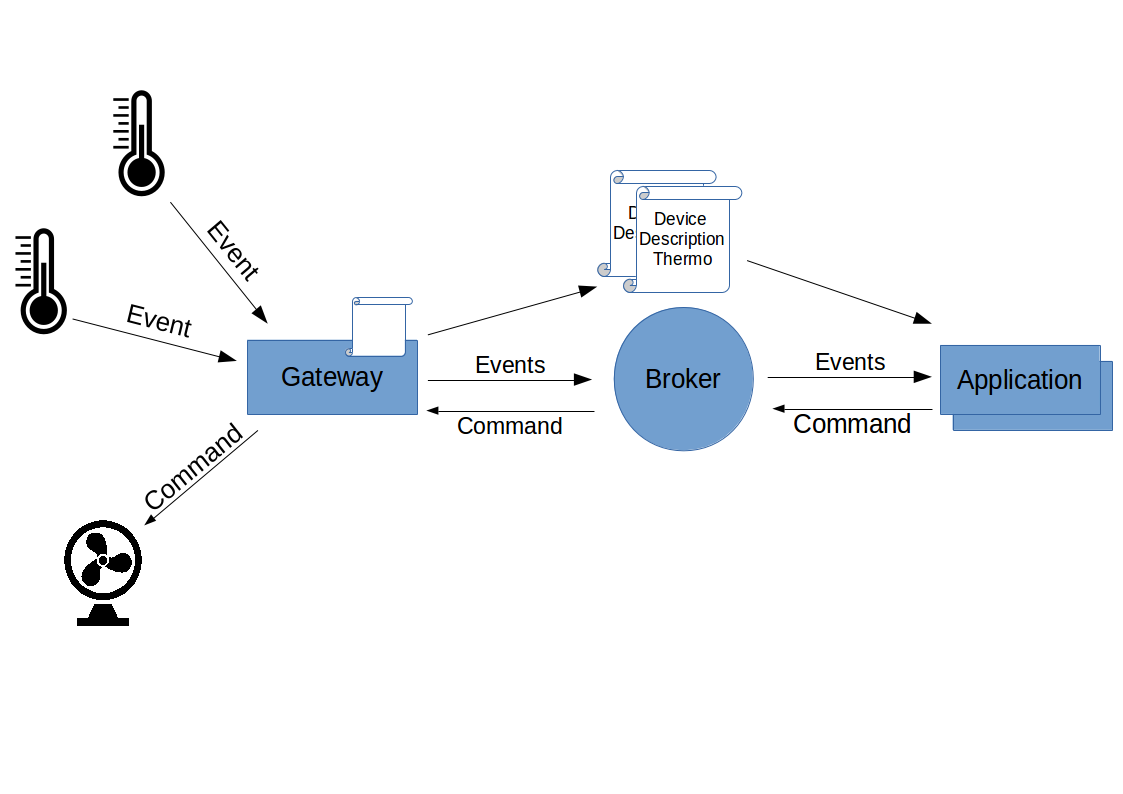
\includegraphics[width=0.8\textwidth]{diag/Overview.png}
	\caption{\label{fig:overview}Übersicht }
\end{figure}


\section{Hierarchie Topics}


Die Topic Hiearachie wird nach folgenden Muster aufgebaut:


\begin{table}[h!]
\begin{tabularx}{\textwidth}{|l|X|l|}

 \hline
 {\bf Level } & {\bf Beschreibung } & {\bf Beispiel } \\ 
 \hline
 0  &   \textbf{Identifikation Anwendung} \newline Eindeutige identifikation der Anwendung.  &    
  ch.bfh.barta3.myApp   \\ \hline
 
 1  &   \textbf{Master Host}  \newline asdf  &     -   \\ \hline

 2  &   \textbf{Gateway (Stack)}   &     -   \\ \hline

 3  &   \textbf{Device Typ} \newline Bezeichnung, um was für einen Typ von Sensor oder Aktor es sich handelt.  &     Temperatursensor   \\ \hline

 4  &   \textbf{Device ID} \newline Da mehrere Devices vom selben Typ im Einsatz sein können, wird auf dieser Stufe mit einer eindeutigen ID der konkrete Sensor resp. Aktor angegeben.   &    mxg   \\ \hline
 
  4  &   \textbf{Device Description} \newline d   &    -   \\ \hline

 5  &   \textbf{Kategorisierung Devicedaten} \newline  Die Eigenschaften und Daten werden in die nachfolgenden drei Teile aufgegliedert.  &     Events, State, Commands   \\ \hline

 6  &   \textbf{Events} \newline  TODO  &     Temperatur   \\ \hline

 6  &   \textbf{State} \newline  TODO  &     Interval   \\ \hline
 
 6  &   \textbf{Commands} \newline  TODO  &   setInterval   \\ \hline
 
\end{tabularx}
\caption{Topic Hierarchie}
\end{table}

\begin{figure}[H]
	\centering
		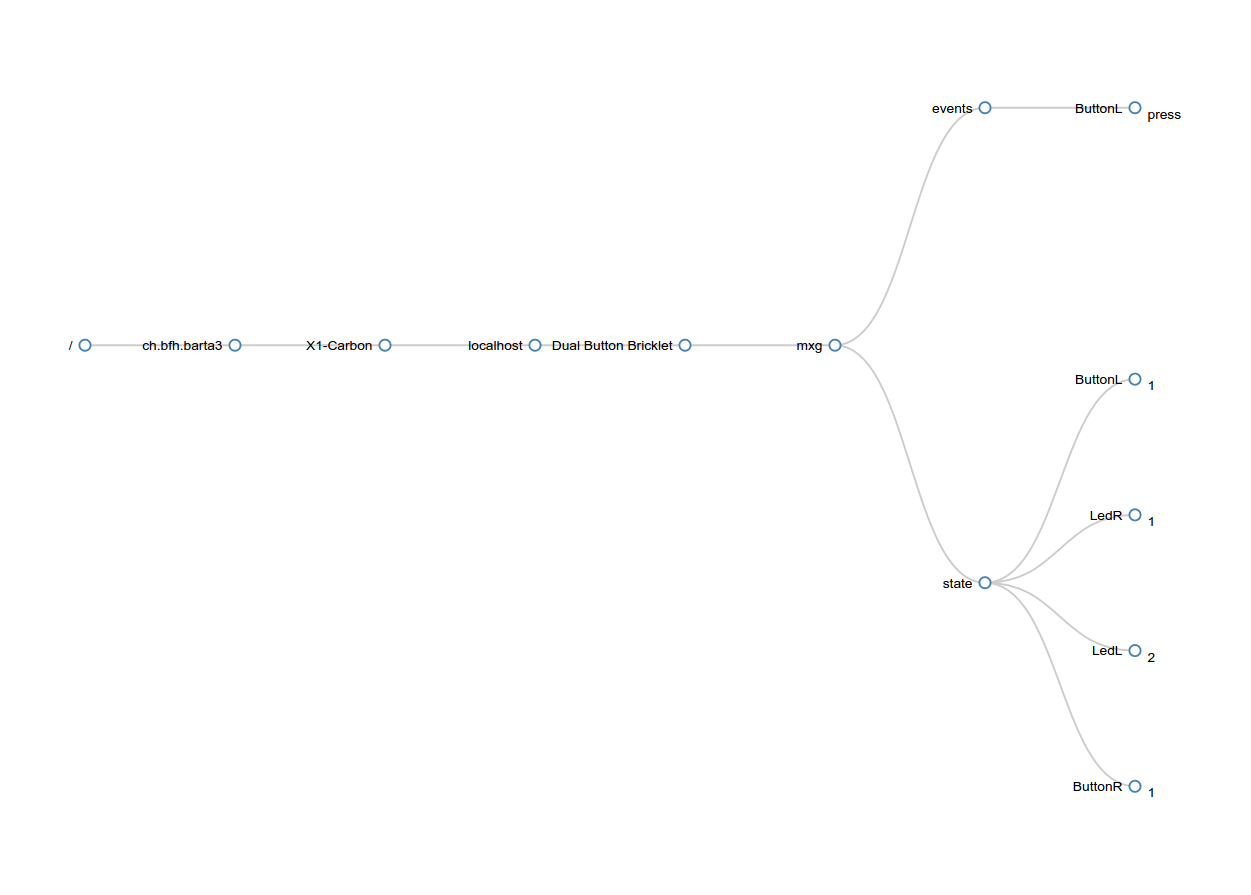
\includegraphics[width=0.8\textwidth]{bilder/TopicHierarchie_Bsp_Dualbutton.png}
	\caption{\label{fig:tempitTopics}Visualisierung MQTT Topics Tinkerforge IR Temperatur Sensor}
\end{figure}

TODO: better diagram



\section{Device Description}

Die Beschreibung eines Device enthält die drei Elemente State, Events und Commands.

\textbf{State} \\
Die State Informationen des Devices werden als Key-Value Paare abgebildet. Der Name der Keys muss eindeutig sein.

\textbf{Events} \\
Ein Device muss beschreiben, welche Events es versendet und was darin enthalten ist.
Ein Event ist folgendermassen aufgebaut:
Name, Liste von Attributen als Key-Value Paare.

\textbf{Commands}